\documentclass{article}
\usepackage[T1]{fontenc}
\usepackage{lmodern}
\usepackage{graphicx}
\usepackage{amsmath,amssymb}
\usepackage[a4paper,margin=2cm]{geometry}
\usepackage[absolute,overlay]{textpos}
\setlength{\TPHorizModule}{1mm}
\setlength{\TPVertModule}{1mm}
\usepackage[indonesian]{babel}
\usepackage{hyperref}
\setlength{\emergencystretch}{2em}
% unit: Halaman 112

\begin{document}

% === Halaman 112 (python/native) ===

• Sebagai contoh, tinjau 3 rotor yang disederhanakan menjadi hanya 6 huruf alfabet:

• Misalkan huruf plainteks D ditekan pada 

keyboard

• Huruf D dienkripsi oleh roto pertama menjadi E

• Huruf E menjadi input untuk rotor kedua, 

dienkripsi menjadi B

• Huruf B menjadi input untuk rotor ketiga, 

dienkripsi menjadi E

• Jadi, huruf D dienkripsi menjadi E

• Setelah D dienkripsi menjadi E, rotor ketiga 

bergeser satu huruf. 

• Jika D dienkripsi kembali, maka hasilnya 

adalah  A

Sumber: https://www.usna.edu/Users/cs/nchamber/courses/ic211/s19/lab/l04/realenigma.html 

112

% deskripsi: gambar native xref 402
\noindent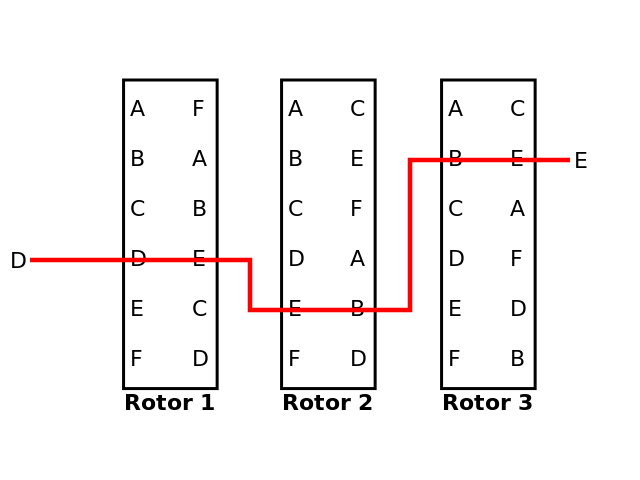
\includegraphics[width=0.85\textwidth]{../../images/python/page_112_img_01.png}

% deskripsi: gambar native xref 403
\noindent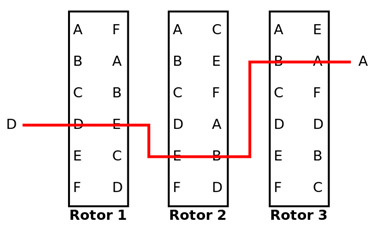
\includegraphics[width=0.85\textwidth]{../../images/python/page_112_img_02.png}

\end{document}
